\documentclass[12pt]{beamer}

\usepackage[utf8]{inputenc}
\usepackage[dutch]{babel}
\usepackage{listings,tabu,tikz,amsmath,xcolor,textcomp,framed}

\definecolor{myblue}{rgb}{0,0,0.7}
\definecolor{mygreen}{rgb}{0,0.5,0}
\definecolor{mygray}{rgb}{0.4,0.4,0.4}
\definecolor{mymauve}{rgb}{0.3,0,0.5}
\definecolor{linkblue}{rgb}{0,0.3,0.5}

\newcommand{\urlb}[1]{{\color{linkblue}\url{#1}}}
\newcommand{\hrefb}[2]{{\color{linkblue}\href{#1}{#2}}}

\lstset{
    language=C++, basicstyle=\footnotesize, frame=single,
    literate=%
        {à}{{\`a}}1
        {â}{{\^a}}1
        {É}{{\'E}}1 {é}{{\'e}}1
        {è}{{\`e}}1
        {ê}{{\^e}}1
        {î}{{\^i}}1,
    commentstyle=\color{mygreen},
    keywordstyle=\bf\color{myblue},
    stringstyle=\color{mymauve},
    showstringspaces=false
}

\beamertemplatenavigationsymbolsempty
\AtBeginSection[]
{
    \begin{frame}
    \frametitle{Inhoudstafel}
    \tableofcontents[currentsection]
    \end{frame}
}

\title{Een eerste probleem oplossen}
\subtitle{UVa 11172 --- Relational Operators}
\author{beOI Training}
\institute{\includegraphics[height=12em]{../share/beoi-logo}}
\date{}

\begin{document}

\maketitle

\begin{frame}
\frametitle{Inleiding}
Dit document legt kort uit hoe je een omgeving opzet om in te programmeren en hoe je je eerste algoritmisch probleem op UVa oplost.

~

De uitleg concentreert zich op een Linux omgeving en het gebruik van de commandoregel. Deze instrumenten zijn krachtig en komen overeen met de beschikbare instrumenten tijdens een wedstrijd, dus is het aangeraden deze een beetje te kunnen gebruiken.

~

Om Linux te gebruiken zijn er meerdere opties, maar de meest eenvoudige oplossing om mee te beginnen is het installeren in een virtuele machine. Voor handleidingen, zoek naar ``Ubuntu installeren op een virtuele machine''\footnote{Sommige instructies in dit document zijn specifiek voor Ubuntu, dus als je geen eigen mening hebt, kies dan best voor deze Linus distributie} op Google
\end{frame}


\section{Vereisten}

\edef\hc{\string:}
\begin{frame}
\frametitle{programmeer omgeving (C++)}
Op Linux:
\begin{itemize}
    \item Installeer de compiler \texttt{g++}: \lstinline[language=bash]|sudo apt install g++|
    \item Gebruik een goede tekst editor: de standaard editor is perfect (gedit, geany, etc.). Meer geavanceerd: vim, emacs.
\end{itemize}

~

Op Windows:
\begin{itemize}
    \item De beste oplossing: installeer Linux (dual boot of VM)
    \item Anders, bekijk Code\hc\hc{}Blocks: \urlb{http://www.codeblocks.org/downloads/binaries}
    \item Download het bestand dat lijkt op \texttt{codeblocks-16.01mingw-setup.exe}
    \item Gebruik \textbf{geen} online IDE! (zeer slechte gewoonte)
\end{itemize}
\end{frame}


\begin{frame}
\frametitle{Online judge}
\begin{itemize}
    \item Online judge = systeem dat code evalueert en het gedrag ervan verifieert op veel voorbeelden
    \item We gebruiken UVA (maak een account aan): \urlb{http://uva.onlinejudge.org}
\end{itemize}
\begin{center}
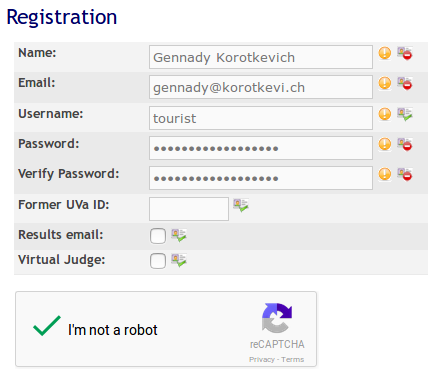
\includegraphics[height=0.45\linewidth]{img/uva-signup}
\end{center}
\end{frame}


\section{Programmeren}

\begin{frame}
\frametitle{Inleiding van het probleem}
Probleemtekst: \urlb{http://uva.onlinejudge.org/external/111/11172.pdf}

\begin{framed}
Some operators checks about the relationship between two values and these operators are called relational operators. \textbf{Given two numerical values} your job is just to \textbf{find out the relationship between them} that is (i) First one is \textbf{greater than} the second (ii) First one is \textbf{less than} the second or (iii) First and second one is \textbf{equal}.
\end{framed}
De context diagonaal lezen (een talent om te ontwikkelen).
\end{frame}

\begin{frame}[fragile]
\frametitle{Invoerformaat}
    De invoer wordt gegeven op \emph{standaard invoer}, alsof iemand het bestand manueel lijn per lijn zou intypen in de console.

\begin{framed}
\textbf{Input}

First line of the input file is an integer $t$ ($t < 15$) which denotes how many sets of inputs are there.
Each of the next $t$ lines contain two integers $a$ and $b$ ($|a|, |b| < 1000000001$).

~

\textbf{Sample input}\\
\texttt{3\\
10 20\\
20 10\\
10 10
}
\end{framed}
\end{frame}

\begin{frame}[fragile]
\frametitle{Input: test cases}
De invoer bestaat vaak uit meerdere test cases die zich in hetzelfde bestand bevinden.

~

Hier is het aantal test cases $t$ gegeven in het begin.
\begin{lstlisting}
#include <bits/stdc++.h>
using namespace std;

int main() {
    int t; // aantal test cases
    cin >> t;
    for (int i=0; i<t; i++) {
        // code hier
    }
}
\end{lstlisting}
\end{frame}

\begin{frame}[fragile]
\frametitle{Input: gegevens}
Nu volstaat het $a$ en $b$ in te lezen.
\begin{lstlisting}
#include <bits/stdc++.h>
using namespace std;

int main() {
    int t; // aantal test cases
    cin >> t;
    for (int i=0; i<t; i++) {
        int a, b; // gegevens
        cin >> a >> b;
        // bereken het antwoord
    }
}
\end{lstlisting}
    Opmerking: \lstinline|cin| laat toe om gehele getallen, floating point getallen en string in te lezen, gescheiden door spaties of op een nieuwe regel.
\end{frame}

\begin{frame}[fragile]
\frametitle{Resultaat en uitvoer}
Nu we $a$ en $b$ hebben, moeten we enkel het resultaat nog berekenen.
\begin{lstlisting}
// in de lus:
if (a < b)
    cout << "<" << endl;
else if (a > b)
    cout << ">" << endl;
else
    cout << "=" << endl;
\end{lstlisting}
    Opmerking: Het is geen probleem om uitvoer te beginnen schrijven voor je alle invoer gelezen hebt.
\end{frame}


\section{Compileren, testen, indienen}

\begin{frame}[fragile]
\frametitle{De console openen}
De uitleg voor de compilatie en het testen concentreren zich op een Linux omgeving in de console.

~

Twee manieren om de console te openen:
\begin{itemize}
\item Openen in de lijst van toepassingen. Typisch heet het ``Terminal'', ``Console'' of ``Shell''
\item Vanaf de verkenner: naar de map navigeren, rechts klikken en ``Open in Terminal'' of gelijkaardig klikken. Voordeel: we zijn direct in de juiste map.
\end{itemize}

~

Wanneer je de console open, geeft een regel tekst de huidige map aan: standaard is dat \lstinline|~|, de map ``Home'', die \lstinline|Documents|, \lstinline|Downloads|, \dots bevat
\end{frame}

\begin{frame}[fragile]
\frametitle{Basiscommando's}
Nuttige commando's:
\begin{itemize}
\item \lstinline|ls|: de inhoud van de huidige map oplijsten
\item \lstinline|cd folder|: naar de submap \lstinline|folder| gaan
\item \lstinline|cd ..|: teruggaan naar de bovenliggende map
\end{itemize}

\begin{center}
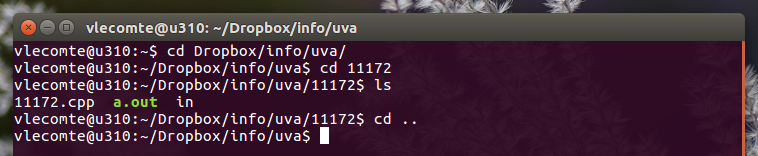
\includegraphics[height=0.17\textwidth]{img/console}
\end{center}

Nuttige toetsen:
\begin{itemize}
\item Tab: de naam van een bestand/map/programma die gedeeltelijk getypt is aanvullen.
\item Pijltje naar boven/beneden: de geschiedenis doorlopen en eerder uitgevoerde commando's herhalen.
\end{itemize}
\end{frame}

\begin{frame}[fragile]
\frametitle{Compileren}
Commando om te compileren:
\begin{lstlisting}[language=bash]
g++ -std=c++11 -Wall -Wextra -Wshadow -O2 a.cpp
\end{lstlisting}
\begin{itemize}
\item \lstinline|g++|: naam van de compiler
\item \lstinline|-std=c++11|: gebruikte C++ versie
\item \lstinline|-Wall -Wextra -Wshadow|: activeer veel waarschuwingen om bugs te vermijden
\item \lstinline|-O2|: compileer het programma om het snel uit te voeren
\item \lstinline|a.cpp|: source code (je moet in de juiste map zijn!)
\end{itemize}
Als alles in orde is, geeft dit geen uitvoer en maakt het het programma \lstinline|a.out| aan. Anders, lees de foutboodschap/waarschuwing, verbeter en probeer opnieuw.

~

Om de naam van \lstinline|a.out| aan te passen, voeg de optie \lstinline|-o andereNaam| toe.
\end{frame}

\begin{frame}[fragile]
\frametitle{Compilatie: pro-tip}
    Raadgeving: voor de volgende regel toe op het einde van \lstinline|~/.bashrc|:
\begin{lstlisting}[language=bash]
alias g="g++ -std=c++11 -Wall -Wextra -Wshadow -O2"
\end{lstlisting}
De naam \lstinline|.bashrc| begint met een punt en is dus standaard verborgen. Om het weer te geven in de verkenner, gebruik Ctrl+H. Het is een gewoon tekstbestand.
\begin{center}
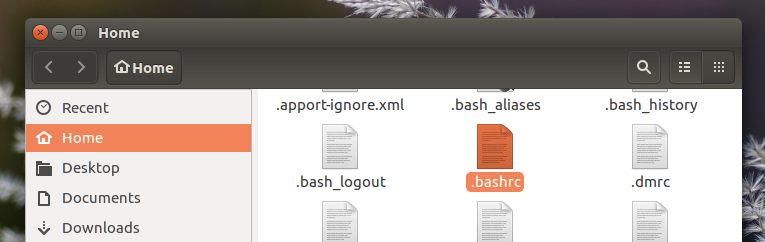
\includegraphics[height=0.2\textwidth]{img/bashrc}
\end{center}

Nadat je de console opnieuw geopend hebt, volstaat het op \lstinline|g a.cpp| te typen om te compileren met alle opties.
\end{frame}

\begin{frame}[fragile]
\frametitle{Testen en debuggen}
    Om het programma uit te voeren, type je gewoon \lstinline|./a.out|. Als je de invoer lijn per lijn geeft, zal het programma die inlezen en daarop reageren.\footnote{Sommige problemen vragen om de invoer tot ``het einde van het bestand'' (EOF) te lezen. Dat kan je aangeven met Ctrl+D.}

~

Om te vermijden dat je de invoer elke keer opnieuw met intypen, kan je deze opslaan in een tekstbestand (bvb. \lstinline|11172.in|, de naam heeft geen belang) en hem automatisch aan je programma geven met het commando \lstinline|./a.out < 11172.in|. Voor grotere programma's is het aangeraden je eigen input te maken.

~

    Gelijkaardig kan je de uitvoer van een programma in een tekstbestand opslaan met \lstinline|./a.out > 11172.out| of zelfs de twee combineren met \lstinline|./a.out < 11172.in > 11172.out|. Het uitvoerbestand wordt aangemaakt als het nog niet bestond.
\end{frame}

\begin{frame}
\frametitle{Indienen en verdict}
Na het testen, is het tijd om je programma in te dienen bij de judge om te verifiëren dat correct en snel genoeg is. Het eenvoudigst is de pagina ``Quick Submit'' in de menu op links in UVa. Voer het nummer van het probleem in, en kies C++11 als taal.

~

Daarna kan je het verdict vinden in ``My submissions'':
\begin{itemize}
\item Accepted: het programma is correct, bravo!
\item Wrong Answer: de uitvoer is fout
\item Time Limit Exceeded: het programma is te traag
\item Runtime Error: het programma is gecrasht
\item Compilation Error: het programma compileert niet
\item Presentation Error: het uitvoerformaat is incorrect
\end{itemize}
\end{frame}

\section{En verder}

\begin{frame}
\frametitle{Selectieproblemen voor beCP}
    Nu je je eerste probleem opgelost hebt, kan je verdergaan met de 9 andere problemen voor de selectie voor stages van beCP. Meer info: \urlb{http://becp.be-oi.be/nl/}

~

    Na $\sim 1$, kan je ook uHunt gebruiken om je UVa statistieken te raadplegen: \urlb{http://uhunt.felix-halim.net}
\begin{center}
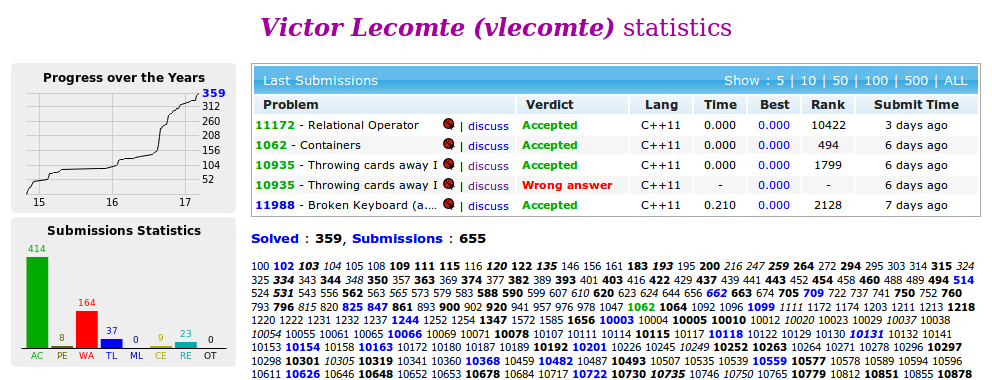
\includegraphics[height=0.3\linewidth]{img/uhunt}
\end{center}
\end{frame}

\begin{frame}
\frametitle{Trainingsmaterialen}
Alle materialen van de beCP training zijn publiek beschikbaar op de site: \urlb{https://github.com/be-oi/beoi-training}
\begin{itemize}
\item Per hoofdstuk geschikt, met duidelijk opschreven onderwerpen
\item Slides van alle lessen
\item Oefeningen verbonden aan de geziene onderwerpen
\end{itemize}

~

Andere sites stellen een nogal compleet programma van lessen en oefeningen voor:
\begin{itemize}
\item \hrefb{http://www.france-ioi.org}{France-IOI} (Frans): trainingssite van het Franse team voor IOI.
\item \hrefb{http://train.usaco.org/usacogate}{USACO} (Engels): idem voor de VS.
\end{itemize}
\end{frame}

\begin{frame}
\frametitle{Platformen en wedstrijden}
Er bestaan nog veel andere sites met oefeningen en wedstrijden:
\begin{itemize}
\item \textbf{\hrefb{http://codeforces.com/}{Codeforces}}: goede problemen en regelmatig wedstrijden
\item \textbf{\hrefb{https://open.kattis.com/}{Kattis}}: qualiteitsproblemen, met aanduiding van niveau\footnote{Soms moet je dit met een korrel zout nemen als het nog niet door veel mensen opgelost is.}
\item \textbf{\hrefb{http://hsin.hr/coci/}{COCI}}: 7 wedstrijden per jaar, erg gericht op IOI
\item \textbf{\hrefb{http://usaco.org}{USACO}}: 4 wedstrijden per jaar, erg gericht op IOI, deelnemen eender wanneer tijdens een weekend
\item \hrefb{https://www.codechef.com/}{CodeChef}: drie wedstrijden per maand, waarvan 1 verspreid over tien dagen
\item \hrefb{https://icpcarchive.ecs.baylor.edu/}{ACM-ICPC Live Archive}: problemen van ACM-ICPC, een universitaire wedstrijd algoritmiek
\item \hrefb{http://www.spoj.com/}{SPOJ}: Enorme bibliotheek aan problemen
\end{itemize}
\end{frame}

\begin{frame}
\frametitle{Boeken rond algoritmiek}
Enkele goede referenties voor competitive programming en algoritmiek in het algemeen:
\begin{itemize}
\item \textbf{\hrefb{https://cses.fi/book.html}{Competitive Programmer's Handbook}} (gratis): Volledig nieuw, maar ziet er goed geschreven en tamelijk volledit uit.
\item \hrefb{https://cpbook.net}{Competitive Programming 3} (betalend): Heel volledig, maar soms moeilijk om te lezen. Bevat problemen voor elk onderwerp, van variabele kwaliteit.
\item \hrefb{http://algs4.cs.princeton.edu/home/}{Algorithms (Sedgewick, Wayne)} (betalend): Een goede referentie rond algoritmiek in het algemeen.
\end{itemize}
\end{frame}

\end{document}
